\section{Mini Pacman}

The performance improvement of I2A over the model-free baseline is most obvious on planning intensive tasks, as for example the atari game MsPacman.
In MsPacman, the player 'pacman' needs to avoid situation where he get enclosed by 'ghosts'. Also the 'ghosts' are not always visible to the player, which results in the nessesarity to predict the current positions of the 'ghosts' to avoid them.
MsPacman is also a path planning problem as a level is sucessfuly finished when 'pacman' has collected all pills.\\

Even though MsPacman would be a nice task to compare I2A with the model-free baseline, it is due to the very long training time of I2A  impossible to train the model with current hardware.
The model-based path of i2a performs in each forward step for each possible action one rollout. Where each rollout consists of n next observation prediction and each observation has the size of a MsPacman input observation, which is 210x160x3 pixel. Even if the observation size is downsampled to 80x80x3 pixel, the number of weights is way to high.\\

As our goal is to verify the performance improvement based on a planning problem and not on a vision problem, a mini version of pacman is used. The mini version is called 'MiniPacman' and has a observation size of 15x19x3 pixel, a image of MiniPacman is depict in Figure \ref{fig:mini_pacman}.
MiniPacman makes the vision problem easier but preserves the reinforcement learning problem.


\begin{figure}[H] 
  \centering   
  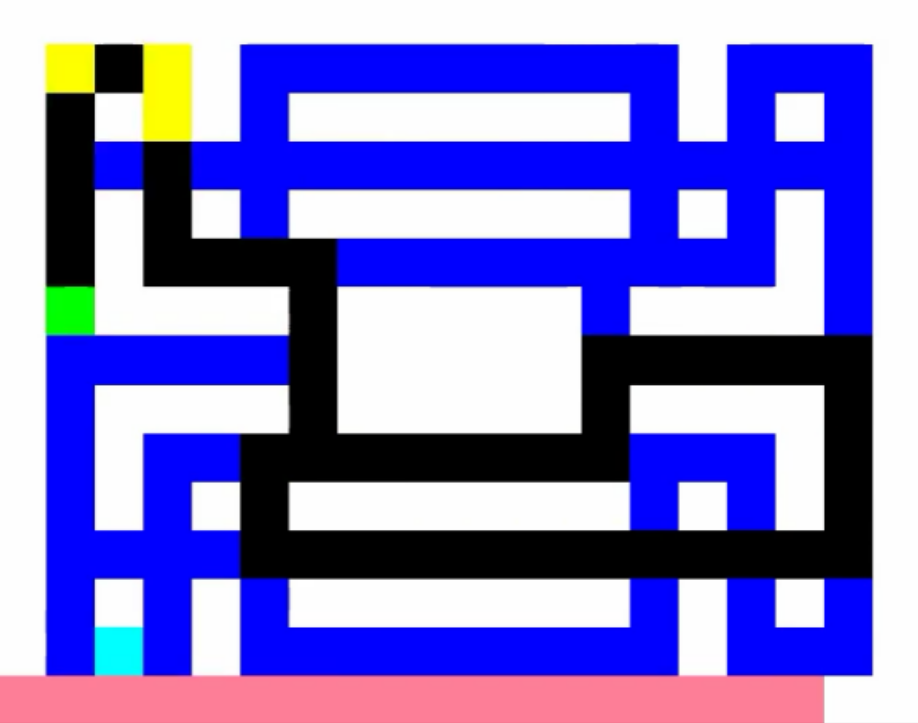
\includegraphics[width=0.5\columnwidth]{./Images/mini_pacman.png}
  \caption{Mini Pacman} 
  \label{fig:mini_pacman} 
\end{figure} 


MiniPacman can be played in different modes. All modes share the same environment but vary in their reward structure and level termination.
In the I2A paper they compared 5 different modes, we due to restricted time and resources only trained I2A in 2 different modes, Regular and Hunt. In the mode Regular a level is cleared when all the food is eaten, in Hunt when all ghosts are eaten or after 80 steps. 
The rewards assoziated with different events are listed in the table below:

\begin{center}
	\begin{tabular}{| c | c | c | c |c | c | }
	\hline
	Task 	& At each step 	& Eating food 
		& Eating power pill & Eating ghost  & Killed by ghost\\
	\hline
	Regular & 0		& 1 	& 2		& 5		& 0 \\
	Hunt	& 0		& 0		& 1		& 10	& -20\\
	\hline
	\end{tabular}
\end{center}

The MiniPacman implementation we used is the same as the one used in the i2a paper and can be found on the github repository of Sebastien Racaniere \cite{MiniPacmanRepo}.


